% !TeX root=../main.tex
\chapter{مروری بر کارهای گذشته}

\section{مقدمه}
در فصل اول مفاهیم پایه و اساسی در مسئله شناسایی فعالیت انسان در تک تصویر با استفاده از شبکه‌های عصبی عمیق و مکانیزم توجه مطرح و بررسی شد و توضیحات مختصری از هربخش داده شد. در این فصل تعدادي
از روش‌های شناسایی فعالیت شناخته شده در این حوزه بررسی شده است. در این فصل مقالات و
الگوریتمهایی که این پایان نامه در راستاي مسیر آنها پیش رفته است و ایده‌ي اصلی این تحقیق بر اساس این
روشها شكل گرفته است، به صورت کامل و با جزییات بیشتري توضیح داده شده است.
در نمودار %
\ref{fig:masir_asli_payan}
 الگوریتم‌های تشخیص فعالیت انسان تقسیم بندی شده است. دسته هایی که تحقیق حال حاضر در آن قرار گرفته با رنگ سبز رنگ مشخص شده اند.
\vspace{8pt}
\begin{figure}[ht]
	\centerline{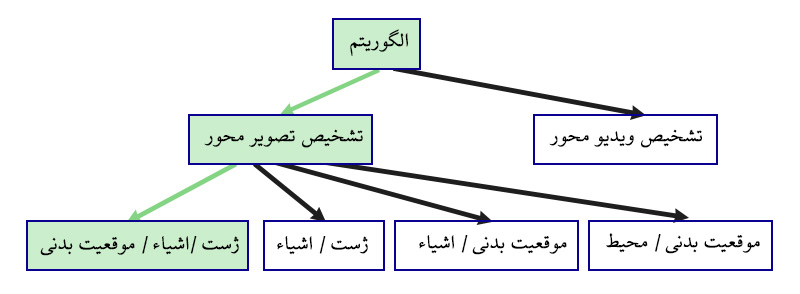
\includegraphics[width=0.8\textwidth]{masir_asli_payan}}
	\caption{دسته بندی الگوریتم های تشخیص فعالیت انسان}
	\label{fig:masir_asli_payan}
\end{figure}
%\vspace{12pt}

\section{تشخیص فعالیت  در تک تصویر}
مطابق با زمینه‌های دیگر در بینایی کامپیوتر، تشخیص فعالیت انسان در تک تصویر از روش‌های سنتی و دستی استخراج ویژگی تکامل یافته تا به روش‌های شبکه عصبی عمیق رسیده است.

در سال 2018 سرلا اس آر و همکارش %
\cite{ActionRec_using_Res_network}
از یک مدل شبکه عصبی عمیق برای کلاس‌‌بندی استفاده کرده اند. آنها بدون درنظر گرفتن هیچ یک از اصلاعات اضافی در تصویر که شامل محیط،‌ ژست و اشیاء می‌باشد، فقط به شکل یک مسئله کلاس‌بندی به موضوع نگاه کرده اند.

در سال 2019 سینا محمدی و همکارانش %
\cite{Ensemble_deep_neu_action_still}
 بهبودی بر شبکه های عصبی با نگاهی به مکانیزم توجه داشته اند. برای غلبه بر کم بود داده ها برای آموزش شبکه‌های کانولوشنی از روش %
\gls{EnsembleLearning}
  استفاده کرده اند. آنها از طریق %
\gls{TransferLearning}
مدل های آموزش دیده قبلی، به مدل های جدید خودشان بهبودی روی دقت داشته اند. همچنین از مکانیزم توجه برای یافتن ارتباط بین اجزای تصاویر در داخل ساختار مدل استفاده شده که موجب افزایش دقت شده است.
 
 در سال 2020 سید سجاد اشرفی و همکارانش %
 \cite{Knowledge_dist_recognition}
 از شبکه %
 \gls{Teacher-Student}
 که جزء روش های %
\gls{KnowledgeDistillation}
 محسوب می‌شود، استفاده کرده اند. در اینکار از یک شبکه بزرگتر برای آموزش یک شبکه کوچکتر کمک گرفته اند. این کار آموزش شبکه کوچکتر را تسریع می‌کند و همچنین باعث می‌شود شبکه در ابتدا مسیر آموزش خود را بداند و از %
\glspl{Loss}
  بزرگ جلوگیری شود. در این کار وابستگی به %
\gls{BoundingBox}
  انسان یا اشیاء وجود ندارد و شبکه می‌تواند بدون درنظر گرفتن %
 \gls{BoundingBox}
   مسیر آموزش خود را طی کند.
  
  در سال 2021 حجت اصغریان و همکارانش %
  \cite{Still_image_action_ensemble}
  مدل یادگیری گروهی بهبود یافته ای که از مکانیزم توجه ویژگی محور بهره می‌برد،‌ استفاده کرده اند. آنها با درنظر گرفتن این واقعیت که مدل روی مجموعه داده‌های کوچکتر، اغلب نتیجه‌ی بهتری نیز می‌دهد، مجموعه داده را به 4 بخش تقسیم کرده اند سپس برای هر بخش یک شبکه کانولوشنی و دسته‌بند جدا درنظر گرفته اند.\\
در کنار این از مکانیزم توجه نیز بهره برده اند که این چهار تا بخش تقسیم شده از مجموعه داده، یکبار باهم مقایسه و ارتباط سنجی شود تا یک ویژگی ترکیب شده از اینها بدست بیاید.

در اغلب این مقالات که ذکر شد، توجه‌ی به ناحیه های کلیدی مانند انسان،‌ اشیاء و ژست به صورت یک بخش مکمل نشده است. اینکار مدنظر ما نیست چون منطقی به نظر نمی‌رسد که اطلاعات مفید تصویر را نادیده بگیریم. بدلیل نداشتن اطلاعات زمانی در تشخیص فعالیت تک تصویر، نادیده گرفتن این اطلاعات دقت تشخیص را کاهش خواهد داد. درهمین‌حین حضور اطلاعات نامرتبط مانند %
\gls{Background}
  و اشیاء نامرتبط منجربه گمراهی شبکه می‌شود.
  
  در سال 2022 پاوان و همکارش %
	\cite{action_sift_key_points}
	از SIFT %
	\LTRfootnote{Scale-Invariant Feature Transform}
	جهت یافتن نقاط کلیدی بدن انسان در تصویر استفاده کردند و از این نقاط بدست آمده برای تشخیص فعالیت بهره بردند.\\
برای شناسایی نقاط برجسته پایدار، تصویر اصلی را با یک تابع گوئسین%
	\LTRfootnote{Guasian}
	ترکیب کردند و لبه‌های مفید از ناحیه انسان را بدست آوردند. از این لبه‌های بدست آمده اطلاعات مهمی بدست ‌می‌آید که در تشخیص فعالیت موثر هستند.این لبه‌ها در تشخیص نقاط اطراف بدن انسان استفاده ‌می‌شود. در نهایت از نقاط کلیدی بدن انسان استفاده کردند تا فاصله اعضای بدن با یکدیگر را محاسبه کنند و درقالب یک بردار ویژگی در روند آموزش ازش استفاده کردند. دراینجا به دلیل استفاده از الگوریتم‌های یادگیری ماشین برای استخراج نقاط،‌ حجم پارامتر‌ها کاهش می‌یابد ولی درعوض دقت چندان مطلوبی بدست نیامده است.
	
	در سال 2023 محمد عبدالهادی %
	\cite{hum_action_behavior_transfer_learning}
	از یادگیری انتقال استفاده کرده است به شکلی که فقط بخشی از شبکه را آموزش دهد و بخش دیگری را قفل کند که وزن‌های مدل در روند آموزش به‌روز نشوند. دراین کار روی مجموعه داده‌ی که برای آموزش استفاده می‌شود بیشتر تمرکز کرده است.\\
	دراین مقاله از یک مجموعه داده‌ی که روی تشخیص فعالیت انسان در ویدیو کارکرد دارد استفاده کرده است و از فریم‌های ویدیو‌‌های این مجموعه داده به عنوان تصاویر جهت آموزش شبکه بهره برده است. درواقع از یک الگوریتمی استفاده کرده است که فریم‌های برتر را از مجموعه داده جدا کند و از آنها در آموزش شبکه استفاده کند. ضعف این مقاله در استفاده از مدل‌های قدیمی برای استخراج ویژگی به جای مدل‌های به روزتر مانند ResNet است.
	
	در سال 2023 آرناب دی و همکارانش %
	\cite{interactions_adaptive_drnet}
	در یک کار متفاوت روی ارتباط انسان با انسان را در یک فریم از ویدیو برای تشخیص فعالیت انسان کار کردند. آنها برای یافتن این ارتباط از یک ماژول توجه AdaptiveDRNet استفاده کردند. سه عدد از این ماژول ها پشت سرهم در داخل بخش استخراج ویژگی قرار دارند تا ترکیب ویژگی‌ها به خوبی صورت گیرد. همچنین در بین لایه‌‌ها از تابع فعال‌ساز Swish استفاده شده است که اصولا همچین تابع فعال‌سازی در اغلب کارها مشاهده نمی‌شود. البته نتایج روی مجموعه ‌داده‌ی %
	\lr{Stanford40}
	چندان رضایت بخش نیست.
	
	در سال 2023 شوآنگ لی یانگ و همکارانش %
	\cite{patch_boxless_action}
	مدلی طراحی کردند که بی نیاز از %
	\glspl{BoundingBox}
	اشیاء و انسان باشد. آنها با قطعه‌بندی تصویر سعی کردند که مدل را طوری آموزش دهند که از خود تصویر اطلاعات ناحیه‌ای که اشیاء یا انسان درآن قرار دارد را درک کند. مراحل استفاده از دو مسیر تشکیل شده است. در مسیر اول ماژول تحریک فعالیت روی کل تصویر اعمال می‌شود که طبق آن،‌ ناحیه‌های مرتبط با فعالیت بازخود بهتری می‌دهند و مقادیر مقادیر بزرگتری تولید می‌کنند. سپس خروجی این بخش روی بخش‌هایی که قطعه‌بندی روی آنها صورت گرفته که به 4 بخش و 16 بخش تقسیم شده اند، اعمال می‌شود. درنهایت خروجی همه این‌ها باهم وارد بخشی می‌شود که قطعه‌‌ها با اندازه‌های متفاوت به صورت دوبه‌دو باهم ارتباط‌سنجی می‌شوند. درنهایت ترکیبی از خروجی‌های پیش‌بینی شده انجام می‌شود و فعالیت مورد‌ نظر تشخیص داده می‌شود.
	
	در سال 2023 ژیارونگ هی و همکارانش %
	\cite{context_enhancment_methodology}
	از یک روش ترکیبی که از مکانیزم %
	\gls{Self-Attention}
	و مکانیزم توجه روی اطلاعات موجود در تصویر بهره می‌برد، استفاده کردند. تصویر پس‌ از استخراج ویژگی وارد ماژول ارتقاء دهنده اطلاعات می‌شود. دراین‌جا ابتدا ماژول %
	\gls{Self-Attention}
	با استفاده از مجموع وزن‌دار،‌ اطلاعات کلی موجود در تصویر را جمع می‌کند و سپس در بخش بعدی از نواحی مختلف که در تعامل باهم هستند، استفاده می‌کند تا ویژگی‌ها را تقویت کند. از این رو، این بخش می‌تواند روی اهمیت هرناحیه از تصویر تاکید کند و جزییات بیشتری از تصویر را کاوش کند. بعد از اینها از دو لایه FC% 
	\LTRfootnote{Fully Connected}
	استفاده کردند که به نتیجه نهایی و تشخیص فعالیت برسند.

\section{روش های مبتنی بر ژست و اشیاء}
این روش ها در این دسته بندی از اطلاعاتی که از ژست انسان و اشیاء در تصویر بدست می‌آید، در تشخیص فعالیت استفاده می‌کنند. استفاده از این اطلاعات می‌تواند بسیار به تشخیص فعالیت کمک کند. کارهای گذشته نشان می‌دهد که بهرمندی از این اطلاعات نتایج مطلوبی به همراه داشته است.

درسال 2010 بنگ پنگ و همکارش %
\cite{ModelingMutual_OB_POSE}
از تعامل بین ژست و اشیاء بهره برده اند. آنها تلاش کرده اند اشیاء که بیشترین ارتباط را با ژست فرد دارد وارد مدل کنند. البته یکسری چالش هایی نیز مطرح شده است. اول اینکه ممکن است اشیاء درتصویر بسیار کوچک باشند و شناسایی این اشیاء کار دشواری است و دوم اشکال مختلف ژست انسان است که بسته به شرایط ممکن است واقعا تشخیص این ژست برای مدل بسیار سخت باشد. با این حال یک مدل گرافیکی از ارتباط بین ژست و اشیاء ارائه داده اند.

در سال 2011 بنگ پنگ و همکارانش %
\cite{HAR_learing_action_part}
از %
\gls{Attributes}
 و %
\gls{Parts}
 مختلف در تصویر استفاده کرده اند. آنها سعی کرده‌اند با ترکیب این دو بخش، مدل یکپارچه را آموزش دهند که به هردو این‌ها توجه کند.\\
 خصصیه، فعل صرف شده آن عمل را نشان می‌دهد. در یک فعالیت مانند "راندن دوچرخه" فعل "راندن" آن خصیصه یا عمل در حال انجام را نشان می‌دهد. "راندن" می‌تواند شامل "راندن موتور" نیز باشد،‌ بنابراین صرف فهمیدن فعل نمی‌تواند به صورت دقیق آن عمل درحال انجام را توصیف کند. بنابراین به بخش اجزاء نیز توجه کرده اند.\\
 اجزاء متشکل از ژست انسان و اشیاء است. دراینجا اشیاء که نزدیک شخص قرار گرفته را به عنوان عامل دیگری برای تشخیص فعالیت درنظر گرفته اند. برای مثال در یک فعالیت مانند "راندن دوچرخه" که درآن "دوچرخه" یک شی نزدیک به شخص است که به صورت دقیق تر فعالیت را نشان می‌دهد.البته دراینجا ممکن است اشیاء واقعا به آن فعالیت درحال انجام ارتباطی نداشته باشد و باعث شود شبکه منحرف شود.\\
 درکنار این ژست را از طریق Poselet%
 \RTLfootnote{یک الگوریتم تشخیص ژست انسان}
  به دست آورده‌اند که در ارتباط با اشیاء قرار دارد. در نهایت از %
\gls{SupportVectorMachine}
 برای کلاس بندی استفاده شده است. درنتیجه‌ی این کار، %
\gls{Dataset}
 \lr{Stanford40}
 را نیز گردآوری و معرفی کردند.
 
 مقاله %
 \cite{Multi_branch_Attention_Recg_still}
 در سال 2017 توسط شیانگ یانگ و همکارانش، به اهمیت اطلاعات %
\gls{Contextual}
  موجود در تصویر اشاره کرده است، اطلاعات جانبی مانند اشیاء در تصویر که مرتبط با انسان است یا ‌%
\gls{Sence}
 که فعالیت در آن درحال انجام است.\\
 همچنین به اهمیت ژست در شناسایی فعالیت پرداخته شده است. به یکی از ایرادهای استفاده از ژست نیز پرداخته است. در تصویر %
\ref{fig:similar_pose_diff}
 هردو ژست یکسان دارند درحالی که فعالیتی که هرکدام انجام می‌دهند متفاوت است. این ایراد و خطا می‌تواند از طریق توجه به اشیای که دردست دارند کاهش یابد. بنابراین از این ایده استفاده شده تا یک الگوریتم ارتباطی بین ژست و اشیاء مرتبط با انسان را طراحی کنند.\\
 \begin{figure}[ht]
 	\centerline{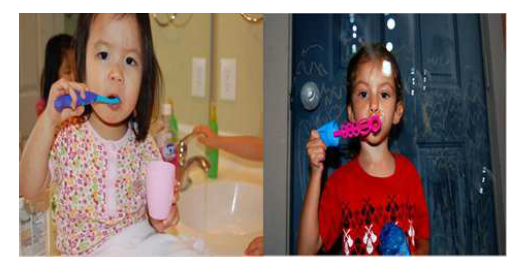
\includegraphics[width=0.7\textwidth]{similar_pose_diff}}
 	\caption{دو تصویر ژست‌های یکسان ولی فعالیت‌های متفاوت را نشان می‌دهد
 		\cite{Multi_branch_Attention_Recg_still}
 		}
 	\label{fig:similar_pose_diff}
 \end{figure}
 برای این منظور از شبکه‌های کانولوشنی (CNN) استفاده شده است تا ارتباط سنجی بین اشیاء و ژست را صورت دهند. در واقع از مفهوم مکانیزم توجه استفاده شده تا این ارتباط سنجی انجام شود. ورودی هایی که برای این شبکه در نظرگرفته شده است ترکیبی از تصویر کامل، اشیاء و اجزای بدن یا همان ژست فرد است که در نهایت از این شبکه عبور می‌کند و یک کلاس‌بندی صورت می‌گیرد.\\ 
 
\section{روش های مبتنی بر موقعیت بدنی و اشیاء}

این روش ها در این دسته بندی از اطلاعاتی که از موقعیت بدنی و اشیاء در تصویر بدست می‌آید، در تشخیص فعالیت استفاده می‌کنند. همانطور که می‌دانید استفاده از اطلاعات اشیاء در جایی که تعامل بین اشیاء و انسان در شکل‌گیری فعالیت نقش دارد، بسیار موثر است. در زیر یک سری کارهایی که توجه روی موقعیت بدنی و اشیاء داشتند اشاره می‌شود.

در سال 2019 لو لی و همکارانش %
\cite{Loss_guided_actv_attention}
در یک کار متفاوت بدون درنظرگرفتن %
\gls{BoundingBox}
 انسان یا اشیاء، از خود تصویر اطلاعات مرتبط با انسان و اشیاء را با کمک مکانیزم توجه، استخراج کرده است. آنها معتقد هستند که %
 \glspl{BoundingBox}
 در داخل خودشان علاوه بر انسان اطلاعات زائد نیز دارند.\\
دراین کار از تصویر یک سری %
\lr{Heatmap}
استخراج شده است که حین آموزش به بخش‌های کلیدی تصویر مانند انسان و اشیاء مرتبط اشاره می‌کند و یک شاخه مجزا درنظر گرفته شده که مکان قرارگیری انسان را تخمین بزند. درشاخه دیگر، از ناحیه‌های برجسته استفاده شده تا محیط و اشیاء نامرتبط نادیده گرفته شود و شبکه دراین شاخه تمرکز بیشتری روی انسان و اشیاء که می‌تواند به فعالیت مرتبط هستند،‌ داشته باشد.

در سال 2020 ونتاو ما %
\cite{Human_object_relation_action}
 از قابلیت مکانیزم توجه درداخل شبکه به شکل موثر استفاده کرده است. از آنجایی که اغلب روش ها برای یافتن ارتباط بین انسان و اشیاء نیازمند یک سری اطلاعات اضافی درمورد نحوه ارتباط انسان با اشیاء هستند،‌ این کار ازاین اطلاعات بی نیاز است. درواقع با بهره مندی از مکانیزم توجه سعی کرده است این ارتباط را شکل دهد. ماژول ارتباط‌سنج انسان-اشیاء که دراین مقاله ذکر شده است این ارتباط را تشکیل می‌دهد.
 ایده اصلی این کار از یک مقاله درمورد استفاده از یک ماژول ارتباط‌سنج درجهت شناسایی اشیاء گرفته شده است %
 \cite{Relation_network_object}
 . این شبکه از دو بخش تشکیل شده است:
\begin{enumerate}
 	\item \textbf{ساختار کلی شبکه:}
برای استخراج ویژگی از شبکه ResNet %
\cite{Resnet_article}
استفاده کرده است. همچنین از آنجایی که اطلاعات انسان و اشیاء را باهم ترکیب کرده اند،‌ به %
\gls{BoundingBox}
هایشان نیز نیاز داشته اند. البته اغلب مجموعه داده‌ها 
\glspl{BoundingBox}
 انسان را فراهم کرده اند اما برای شناسایی 
\glspl{BoundingBox}
  اشیاء از Faster R-CNN استفاده شده است.\\
روش کار به این صورت است که در ابتدا از چهار بلوک کانولوشنی برای استخراج ویژگی سطح پایین تصویر استفاده می‌شود. سپس یک RoI Pooling برای استخراج ویژگی دقیق‌تر به کمک %
\glspl{BoundingBox}
 بر روی ناحیه مورد نظر اعمال می‌شود. از این به بعد شبکه به دو شاخه تقسیم می‌شود.\\
شاخه اول مربوط به ویژگی‌ها و %
\glspl{BoundingBox}
 انسان و شاخه دوم مسیر ویژگی‌ها و %
 \glspl{BoundingBox}
  اشیاء را دربر می‌گیرد. با ورود این دوشاخه به ماژول ارتباط‌سنج،‌ وزن دهی این دو انجام می‌شود و در انتها از روی امتیازات بدست آمده کلاس‌بندی صورت می‌گیرد.
	\vspace{20pt}
 	\item \textbf{:ماژول ارتباط‌سنج انسان-اشیاء}
 هدف از طراحی این بخش بهبود خصیصه‌های فعالیت درحال انجام توسط انسان است. همچنین ویژگی‌های اشیاء مرتبط با انسان را پررنگ تر می‌کند که شبکه بتواند در جاهایی که اشیاء منجربه تفاوت در فعالیت می‌شود را تشخیص دهد. (مانند تصویر %
\ref{fig:similar_pose_diff}
 که مسواک یا حباب ساز تفاوت فعالیت را مشخص می‌کند).\\
\end{enumerate}
 البته موضوعی که اینجا درنظر گرفته نشده است،‌ ژست انسان است مخصوصا وجود اشیاء مرتبط که در تشخیص فعالیت تاثیر به سزایی دارد.
  
	در سال 2023 شوآنگ لیانگ و همکارانش %
\cite{relation_with_free_obj}
کار %
\cite{Human_object_relation_action}
را بهبود دادند. آنها به‌ جای استفاده از شبکه جدا جهت استخراج %
\gls{BoundingBox}
اشیاء، از یک ماژول در داخل ساختار شبکه استفاده کردند که کار استخراج ویژگی و شناسایی ناحیه اشیاء را انجام دهد. آنها به دو ضعف در کار قبلی اشاره کردند که دراین مقاله پوشش داده اند. یکی آموزش مدل است که نیازمند در دست داشتن ناحیه‌های اشیاء است و دیگری ارتباط بین انسان و اشیاء درداخل ماژول ارتباط‌سنج است که به طور کامل در روند آموزش این ارتباط بین انسان و اشیاء یافت نمی‌شود.\\
به همین منظور از یک ماژول جدا جهت یافتن اشیاء استفاده کردند. این مدل را طوری ساختن که در روند آموزش تنها با دراختیار داشتن برچسب نوع فعالیت مدل آموزش ببیند و پارامتر‌ها طوری به روز شوند که اشیاء مرتبط با فعالیت در هنگام تشخیص فعالیت شناسایی شوند. درواقع با این کار شبکه طوری آموزش میبیند که اشیاء با فعالیت درحال انجام درارتباط باشند.
\section{روش های مبتنی بر موقعیت بدنی و ژست}

این روش ها در این دسته بندی از اطلاعاتی که از موقعیت بدنی (کل انسان در تصویر) و ژست در تصویر بدست می‌آید، در تشخیص فعالیت استفاده می‌کنند. استفاده از این اطلاعات می‌تواند دقت کارمان را در تشخیص فعالیت بالا ببرد. کارهای گذشته نشان می‌دهد که بهرمندی از این اطلاعات نتایج مطلوبی به همراه داشته است.

در سال 2017 ژیچن ژاو و همکارانش %
\cite{Single_image_semantic_body}
از اجزای بدن که می‌تواند مفهومی در فعالیت درحال انجام داشته باشد استفاده کردند. برای مثال شخصی که درحال "ریختن آب در لیوان" است و عینک نیز زده است، توجه به سر و عینک می‌تواند شبکه را گمراه کند. درحالی که توجه اصلی فعالیت رو "ریختن آب در لیوان" است که با دست انجام می‌شود. البته این موضوع را نیز درنظر گرفته اند که حالت سر زمانی که رو به پایین است،‌ نسبت به زمانی که سربه رو به بالا است فعالیت متفاوتی را می‌تواند شکل دهد. زمانی که سر رو به بالا است احتمال انجام فعالیت "نوشیدن آب" بیشتر است.\\
این مقاله نیز از این مفهوم استفاده کرده است تا شبکه را طوری طراحی کند که تمرکز روی بخش‌های موثر بدن در انجام فعالیت باشد. برای این منظور ابتدا %
\gls{Keypoints}
بدن را استخراج کردند سپس با کمک این نقاط،‌ ناحیه های بدن را از تصویر بریده و به شبکه دادند تا در این فرآیند از این ناحیه‌ها استفاده شود.  این کار موجب می‌شود شبکه وزن دهی مناسبی به اجزای بدن،‌ درهر فعالیت داشته باشد.
 
 در سال 2020 بیشان باندری %
 \cite{Body_part_aware_multitask_act}
 یک روش چند منظوره برای تشخیص فعالیت ارائه داده است. دراین ساختار داشتن نقاط کلیدی بدن یا %
\gls{Label}
  فعالیت،‌ برای شبکه کافی است و نیازی به داشتن هردو نیست. این کار بی نیاز از داشتن %
  \gls{BoundingBox}
  انسان، اشیاء و ژست است و خود شبکه تمرکز می‌کند که این بخش ها را پیدا کند. البته لازم به ذکر است که دراینجا شبکه بیشتر روی ژست و اجزای بدن تمرکز دارد تا اشیاء.\\
  دلیل اصلی اینکه روی اشیاء تمرکز ندارند این است که اعتقاد دارند زمانی که ناحیه اجزایی که درفعالیت موثر است را مشخص می‌کنیم، اشیاءی که در ارتباط با انسان هستند نیز در این ناحیه قرار می‌گیرند. برای مثال زمانی که ناحیه "دست" مشخص می‌شود، "لیوان" نیز دراین ناحیه قرار می‌گیرد. البته ممکن است اشیاء از ناحیه مشخص شده اجزای انسان بزرگتر باشد و باعث درک غلط شبکه شود.\\
ویژگی‌های تصویر را با استفاده از شبکه %
 \lr{HRNet}
 \cite{HRNet_network}
  که یک شبکه قدرتمند در زمینه استخراج ویژگی با %
\gls{MutliResolution}
   با تمرکز بر ژست انسان است،‌ استخراج کرده است. شبکه ای که طراحی کردند از 3 شاخه تشکیل شده است:\\
  1- شاخه اول مسیر ویژگی روی کل تصویر است. دراین مسیر ویژگی کمترین وضوح استخراج شده از تصویر، مورد استفاده قرار گرفته است. \\
  2- شاخه دوم مسیر %
\gls{Analysis}
  اجزاء مهم تصویر مانند انسان و پس‌زمینه است. دراین شاخه از تمام وضوح ویژگی و همچنین از اجزای بدن استفاده می‌شود تا به نوعی مکانیزم توجه بازسازی شود. توجه اصلی اینجا روی ژست در ترکیب با کل تصویر است.\\
  3- شاخه نهایی روی اجزاء مهم بدن مانند "سر، دست، پا و..." است. این اجزاء در ترکیب با ویژگی ژست انسان یک بهبود بسیارخوب درنتیجه حاصل کرده است.
  
  در سال 2020 یانگ لی و همکارانش %
  \cite{Recognition_fusing_mutple_cue}
  یک %
\gls{UnifiedStructure}
  از مدل شبکه های کانولوشنی با توجه روی ساختار بدنی و ژست انسان در تصویر ارائه کرده اند. برای اینکه کل اجزای بدن را بررسی کنند از دو شاخه و مسیر استفاده کردند.
  \begin{enumerate}
  	\item \textbf{(\gls{BodyStructureExploration})}
  	نشانه های بدن انسان، اطلاعات ارزشمندی برای درک ساختار بدن به ما می‌دهد. ازطرفی هم، نقاط کلیدی بدن محل قرارگیری اجزای بدن در تصویر را خود دارد. از نقاط کلیدی در ساخت %
\gls{Skeleton}
  	انسان که ویژگی کلی بدن انسان را توصیف می‌کند،‌ استفاده ‌می‌شود.
 \gls{Skeleton}
  	 به نوعی نگاه %
\gls{Global}
  	به بدن انسان دارد برای این بخش مسیر %
\gls{LimbAngleDescriptor}
\lr{(LAD)}
  	 تشکیل می‌شود که این ساختار 
  	  \gls{Skeleton}
  	  را در شبکه پیاده سازی کند. همچنین مسیر %
  	 \gls{StructuralBodyParts}
  	 \lr{SBP}
  	 یک نگاه %
  	 \gls{Local}
  	 به اجزای بدن دارد تا ویژگی‌های محلی هم وارد چرخه شود. مانند بخش LAD در این مسیر نیز، از نقاط کلیدی بدن استفاده می‌شود تا نواحی با اندازه مشخص از اجزای بدن از تصویر بریده شود و به عنوان یکی از ورودی های بخش دسته‌بندی کلاس (AC) در روند کلاس‌بندی شرکت کند.\\
  	 به دلیل اینکه ممکن است اندازه شخص درتصویر متفاوت باشد باید با درنظر گرفتن ارتفاع شخص در تصویر،بخش ها بریده شود. به همین منظور از تکنیک %
  	 \gls{Thresholding}
 استفاده می‌شود.
  	\item \textbf{(\gls{ActionClassification})}
  	  با ساختار و خروجی هایی که از طریق نشانه های بدن بدست آمده،‌ کلاس بندی نهایی انجام می‌شود. برای این منظور سه شاخه درنظر گرفته می‌شود که ویژگی های بدست آمده کامل در روند تشخیص فعالیت نقش داشته باشند. هرکدام ازاین شاخه های بخش های مختلفی از تصویر را دربرمی‌گیرد.\\
 شاخه اول،‌ از کل ویژگی های بدست آمده از تصویر بهره می‌برد. شاخه دوم از اجزای بدن که از بخش SBP بدست آمده است،‌ برای کلاس بندی استفاده می‌کند و شاخه سوم به ویژگی 
  \gls{Skeleton}
  بدن که از بخش LAD محاسبه شده است توجه دارد. این سه بخش در تعامل باهم در یک روند امتیاز‌دهی شرکت می‌کنند و با ترکیب شدن امتیازات این سه بخش یک تشخیص فعالیت دقیق تری صورت می‌گیرد. 
  \end{enumerate}
در این پایان نامه نیز از این نوع نگاه به ژست، که درترکیب با موقعیت بدنی منجربه نتیجه مطلوب می‌شود استفاده شده است.
   
   	در سال 2024 ژین بیا لو و همکارانش %
   \cite{a_key_points_assisted_net}
   شبکه‌ای طراحی کردند که از دو مسیر برای استخراج ویژگی بهره می‌برد. مسیر اول اطلاعات کلی از تصویر را با شبکه عصبی کانولوشنی استخراج می‌کند. دراین مسیر از شبکه EfficientNet با اعمال تغییراتی استفاده شده است. مسیر دوم،‌ اطلاعات کمکی و اضافی را از تصویر استخراج می‌کند. این اطلاعات کمی از ژست استفاده می‌کند و در داخل ماژول طراحی شده،‌ که شامل یک سری لایه‌های کانولوشنی است ترکیب می‌شود. برای تخمین ژست نیز از OpenPose استفاده کردند.\\
   جهت افزایش کارایی شبکه از یادگیری انتقالی نیز استفاده کردند. به این صورت که یک شبکه بزرگتر انتخاب کردند و وزن‌‌های شبکه اصلی را که قرار‌ است کار تشخیص فعالیت را انجام دهد، با وزن های شبکه بزرگتر در ابتدای آموزش جایگزین شده است. 
   
   در سال 2024 پاوان و همکارش %
   \cite{shape_orbicular_grid_action}
   روی ناحیه بدن انسان تمرکز کرده و پس زمینه را حذف کردند. چون دریک فعالیت اجزای بدن انسان است که موجب می‌شود فعالیت انسانی صورت گیرد. دراین مقاله نیز روی موقعیت بدنی و ژست شخص جهت تشخیص فعالیت تمرکز کردند.\\
   ابتدا تصویر را به تصویر سطح خاکستری تبدیل کردند و با %
   \gls{Thresholding}
   ، اشیاء یا انسان را از پس زمینه جدا کردند. با استفاده از الگوریتم Canny لبه‌ها را استخراج کردند. سپس از این لبه‌‌ها به انسان و اشیاء متصل به انسان رسیدند. سپس از مرکز این تصویر یک سری بخش‌هایی را به صورت دایره‌ای وار بریدند و بادرکنارهم گذاشتن این بخش‌ها تخمینی از فعالیت انجام دادند.
   
\section{روش های مبتنی بر ژست، اشیاء و موقعیت بدنی}
روش های موجود در این دسته بندی از اطلاعاتی که از موقعیت بدنی، اشیاء و ژست در تصویر بدست می‌آید، در تشخیص فعالیت استفاده می‌کنند. تصویری که شامل فعالیت درحال انجام است هر سه این اطلاعات را دارد. البته در مواردی ممکن است اشیاء وجود نداشته باشد مانند "دویدن" ولی در اکثر مواقع اشیاء و محیط حضور دارند. با این حال مقالات زیر از این سه بخش درکار خود سود برده اند که به چند تایی از این ها می‌پردازیم.

 در سال 2018 هاو شو فانگ و همکارانش %
\cite{Pairwise_bodypart_att_2018}
به صورت خاص محور روی اعضایی از بدن که با اشیاء مرتبط با فعالیت، در تعامل هستند توجه کرده اند. در یک فعالیت مانند "نوشیدن آب" به لیوان آب و همچنین "دست" و "بازو" که لیوان را نگه داشته توجه شده است. این نوع نگرش منجر شده که از مکانیزم توجه در این کار استفاده شود. روشی که استفاده کردند از هردو اطلاعات گلوبال یا کلی و محلی بهره می‌برد. اطلاعات کلی تصویر شامل انسان، صحنه ای که فعالیت درآن درحال انجام است و اشیاء می‌شود. این نوع از ساختار باعث ترکیب هرسه این اطلاعات می‌شود و یک خروجی کلی ارزشمند از فعالیت می‌دهد.\\
برای اطلاعات محلی که ایده اصلی و پیشنهاد مقاله است،‌ از یک ماژول که به صورت جفت، اجزاء بدن را دریک مکانیزم توجه بررسی می‌کند،‌ استفاده شده است. این کار ارتباط بین ویژگی های محلی و هرجزء بدن را پیدا می‌کند. درنهایت پس از ترکیب این ویژگی ها،‌ چند تا دسته برتر انتخاب شده و در ترکیب دوباره با ویژگی های کلی،‌ وارد مرحله کلاس‌بندی می‌شود.

در سال 2021 سید سجاد اشرفی %
\cite{action_multi_att_weakly}
با توجه به اینکه فعالیت درحال انجام در یک محیطی انجام می‌گیرد، یک سری ناحیه‌های برجسته را از این محیط استخراج کرده است. ازآنجایی که هیچ مرز مشخصی در محیط برای این ناحیه‌های برجسته وجود ندارد،‌ استخراج این ناحیه‌ها با چالش هایی همراه بوده است. برای غلبه براین چالش یک روش پیشنهادی به نام شبکه هدایت شده دارای چندین مکانیزم توجه به صورت هدایت شده معرفی شده است که بتواند چندین ناحیه برجسته را همزمان تشخیص دهد.
 برای اینکه شبکه بتواند روی این ناحیه‌ها تمرکز کند، از روش معلم-دانش آموز برای تقطیع دانش بهره برده است. \\
 برخی از روش‌ها که گفته شد باتوجه به اطلاعات اضافی مانند اشیاء و ژست به شبکه در امر تشخیص فعالیت کمک می‌کنند. استفاده از این اطلاعات برای شبکه سودمند است ولی نیازمند یک سری الگوریتم‌های پیچیده برای تخمین ژست و شناسایی اشیاء است. همچنین ناحیه‌های برجسته، اطلاعاتی از ژست و اشیاء را درخودشان دارند زیرا ناحیه‌های مهمی که فعالیت درآن بخش درحال انجام است،‌ شامل ژست و اشیاء مرتبط با فعالیت نیز می‌شود.\\
 همچنین این کار روی چندین ناحیه برجسته،‌ به جای یک ناحیه توجه می‌کند. دلیلش هم این است که درفعالیتی که رخ می‌دهد،‌ ممکن است چندین شیء و یا ناحیه در شکل‌گیری این فعالیت نقش ایفا کنند بنابراین باید همه این ناحیه‌ها را در تصمیم‌گیری لحاظ کرد.\\
شناسایی چندین ناحیه برای شبکه کار مشکلی است و استفاده از یک هدایت کننده کارمعقولی است بنابراین استفاده از مکانیزم توجه دراینجا موثر بوده است. همچنین از یک شبکه معلم-دانش آموز استفاده شده که این مکانیزم توجه که درشاخه دانش آموز قرار می‌گیرد، به شکل درستی آموزش ببیند. شبکه معلم بدلیل قدرتمند بودن نسبت به شبکه دانش آموز،‌ بهترین نواحی را استخراج می‌کند که دربخش شبکه دانش آموز بسیار کمک کننده است.\\
ساختار پیشنهادی این مقاله،‌ استفاده از %
\gls{Function}
 خطاهای
کمکی در آموزش شبکه و Kmeans%
\RTLfootnote{یک الگورتیم بدون ناظر برای خوشه‌بندی می‌باشد}
برای پیداکردن یک سری نواحی برجسته برای %
\gls{BoundingBox}
 می‌باشد. تابع‌های خطا درهر بخش وظیفه‌ی خاص خود را دارند. در یک شاخه یک کمک کننده براش شناسایی اشیاء و نواحی برجسته در تصویر که در ارتباط با فعالیت است، نقش ایفا می‌کند. در شاخه دیگر ناحیه‌ای که انسان قرار دارد را تشخیص می‌دهد و در شاخه آخر به عنوان کلاس‌بند دراین ساختار حضور دارد.

در سال 2022 ژیانگتاو ژنگ و همکارانش %
\cite{Human_action_multiple_s_clue}
یک رویکردی پیشنهاد داده اند که از روی چندین نشانه از روی اطلاعات ثابت تصویر بدون نیاز به %
\glspl{BoundingBox}
 انسان و اشیاء، می‌تواند یک تشخیص مناسب انجام دهد.\\
برای تشخیص فعالیت سه عامل و نشانه در تصویر وجود دارد،‌که اغلب از این سه نشانه برای تشخیص فعالیت استفاده می‌شود:

\textbf{1- اجزاء احاطه شده:}
اجزاء احاطه شده می‌تواند شامل کل اجزاء صحنه در تصویر مانند پس زمینه‌ای که فعالیت درآن شکل گرفته است یا کل تصویر باشد.
 
 \textbf{2- اجزاء انسان:}
 اجزاء انسان می‌تواند شامل ژست یا موقعیت بدنی انسان باشد که همیشه یکی از عوامل متمایز کننده نوع فعالیت بوده است.
 
 \textbf{3- اجزاء مرتبط با فعالیت:}
می‌تواند شامل اجزاء مختلف مانند اشیاء مرتبط با انسان یا اشیاء در تعامل با فعالیت،‌ که درکنار موقعیت بدنی فعالیت درحال انجام را نشان می‌دهد، باشد. برای مثال "در دست گرفتن گوشی" در فعالیت "عکس گرفتن"  و یا "دوچرخه" در فعالیت "دوچرخه سواری". این بخش در تشخیص فعالیت بسیار موثر است.\\
این مقاله نیز مانند مقاله %
\cite{action_multi_att_weakly}
از %
\gls{BoundingBox}
 انسان و اشیاء در داخل شبکه استفاده نکرده است و باکمک مکانیزم توجه سعی می‌کند این نواحی را پیدا کند. ازاین رو رویکردی که پیشنهاده شده است از شبکه ای برای یافتن چندین نشانه فقط از روی اطلاعات موجود در تصویر استفاده ‌می‌شود. دو مسیر اصلی وجود دارد:\\
اول یک مسیر ویژگی‌های اصلی اجزای بدن انسان مانند ژست و موقعیت بدنی را استخراج می‌کند. این بخش فقط از روی برچسب اصلی فعالیت این عمل را انجام ‌می‌دهد. بعد از این ویژگی‌های بدست آمده وارد یک بخش با سه شاخه می‌شود که سه عاملی که بالا گفته شد را در تصویر تشخیص دهد. این کار نتایج مطلوبی داشته و دقت 93\% نیز بدست آمده است که نسبت به روش‌هایی که از %
\glspl{BoundingBox}
 آماده استفاده کردند کمتر است.
\section{جمع بندی فصل}

دراین فصل روش‌های ارائه شده در حوزه تشخیص فعالیت که براساس تک تصویر عمل ‌می‌کنند مورد بررسی قرار گرفتند. در حوزه تشخیص فعالیت تک تصویر سه بخش اصلی موقعیت بدنی، ژست و اشیاء نقش مهمی برای مدل جهت شناخت فعالیت درحال انجام دارد که مقاله‌های معتبر مرتبط در این بخش بررسی شدند.

مقالات مختلف زیادی دراین زمینه منتشر شده است که هرکدام به جنبه‌های از استفاده این بخش ها پرداختند با این حال دربعضی از این مقالات ژست و اشیاء نادیده گرفته شدند. در بعضی از مجموعه داده‌ها اشیاء نقش پررنگی در تشکیل آن فعالیت دارند. دراین نوع مجموعه داده‌ها مقالات مربوطه که اشیاء را نادیده می‌گیرند عملکرد به مراتب ضعیف‌تری داشته اند همچنین درمجموعه داده‌های دیگر ژست عامل اصلی شکل گیری آن فعالیت است و روش هایی که ژست را نادیده گرفته اند در این پیش بینی این فعالیت ها عملکرد ضعیفی داشتند.

بعضی موارد که از اطلاعات ازپیش‌آماده مانند ناحیه‌ی انسان و اشیاء بی‌نیاز بودند هم بررسی شدند. البته الگوریتم‌های مختلف بسیاری برای بدست آوردن این ناحیه‌ها وجود دارد که در روش پیشنهادی از این الگوریتم‌ها برای بدست آوردن این ناحیه‌ها استفاده می‌شود. درکناراین،‌ اکثر مجموعه داده‌ها در کاربرد تشخیص فعالیت،‌ اطلاعات ناحیه اشیاء و انسان را دراختیارمان قرار می‌دهند و دراین پایان نامه فقط نقاط کلیدی انسان با الگوریتم هایی بدست می‌آید.

در فصل بعد،‌ با بررسی نقاط ضعف و قوت روش‌های مختلف و همچنین استفاده از بخش‌های موثر و مفید معرفی شده، راهکار جدیدی برای ترکیب ویژگی‌های بدست آمده از تصویر در جهت تشخیص فعالیت انسان معرفی خواهد شد.
